\section{Server and Client Implementation Deep Dive}
\label{sec:server_client}

While the machine learning microservice provides the core anomaly probability, the overall operational efficacy of HormuzWatch depends on the high-concurrency Go ingestion backend and the real-time React 19 tactical client.

\subsection{Go Backend Engine: Telemetry Ingestion and Composite Fusion}
The Go backend (\texttt{server/}) operates as a high-throughput, low-latency concurrent processing daemon.

\subsubsection{Composite Threat Intelligence Fusion Formulation}
A central innovation in HormuzWatch is the multi-factor risk fusion algorithm defined in \texttt{server/internal/intelligence/composite.go}. Rather than permitting the machine learning model to act as an unconstrained single point of failure, the platform fuses three distinct analytical dimensions:
\begin{equation}
\text{FinalScore} = \operatorname{round}\left( 0.40 \cdot S_{\text{Rule}} + 0.40 \cdot S_{\text{ML}} + 0.20 \cdot S_{\text{Geo}} \right)
\end{equation}
where:
\begin{itemize}[leftmargin=*]
    \item $S_{\text{Rule}} \in [0, 100]$: Deterministic rule heuristic score computed by \texttt{anomaly.Score()}, evaluating speed drops, dead reckoning jumps, and AIS transponder gaps.
    \item $S_{\text{ML}} \in [0, 100]$: Calibrated anomaly probability generated by the Python ensemble microservice.
    \item $S_{\text{Geo}} \in [0, 100]$: Geospatial proximity risk score generated by \texttt{GeoStore.ScoreForLocation()}, assessing distance to disputed islands (Abu Musa, Greater and Lesser Tunbs), military exclusion zones, and historical attack sites.
\end{itemize}
The resulting integer threat score ($[0, 100]$) maps directly to standardized operational severity tiers:
\begin{equation}
\text{Severity} = 
\begin{cases}
\text{Low} & \text{if } \text{FinalScore} \le 30 \\
\text{Medium} & \text{if } 31 \le \text{FinalScore} \le 60 \\
\text{High} & \text{if } 61 \le \text{FinalScore} \le 80 \\
\text{Critical} & \text{if } \text{FinalScore} > 80
\end{cases}
\end{equation}

\subsubsection{Model Version Provenance}
To support strict operational audit trails, the gRPC response from \texttt{grpc\_server.py} populates \texttt{resp.GetModelVersion()}. This version string is preserved by the Go client through \texttt{MLExplanation} and embedded directly into the serialized \texttt{ThreatAssessment}, guaranteeing that operators can trace which exact model artifact generated a given threat assessment.

\subsection{Client-Side Tactical Interface: React 19 and Leaflet Engine}
The frontend application (\texttt{client/}) is engineered for command-center operations environments, utilizing React 19, TypeScript, and React Router v7.

\subsubsection{Tactical Geospatial HUD}
Figure~\ref{fig:tactical_map} illustrates the tactical map interface displaying live maritime contacts transiting the Strait of Hormuz:
\begin{figure}[htbp]
\centering
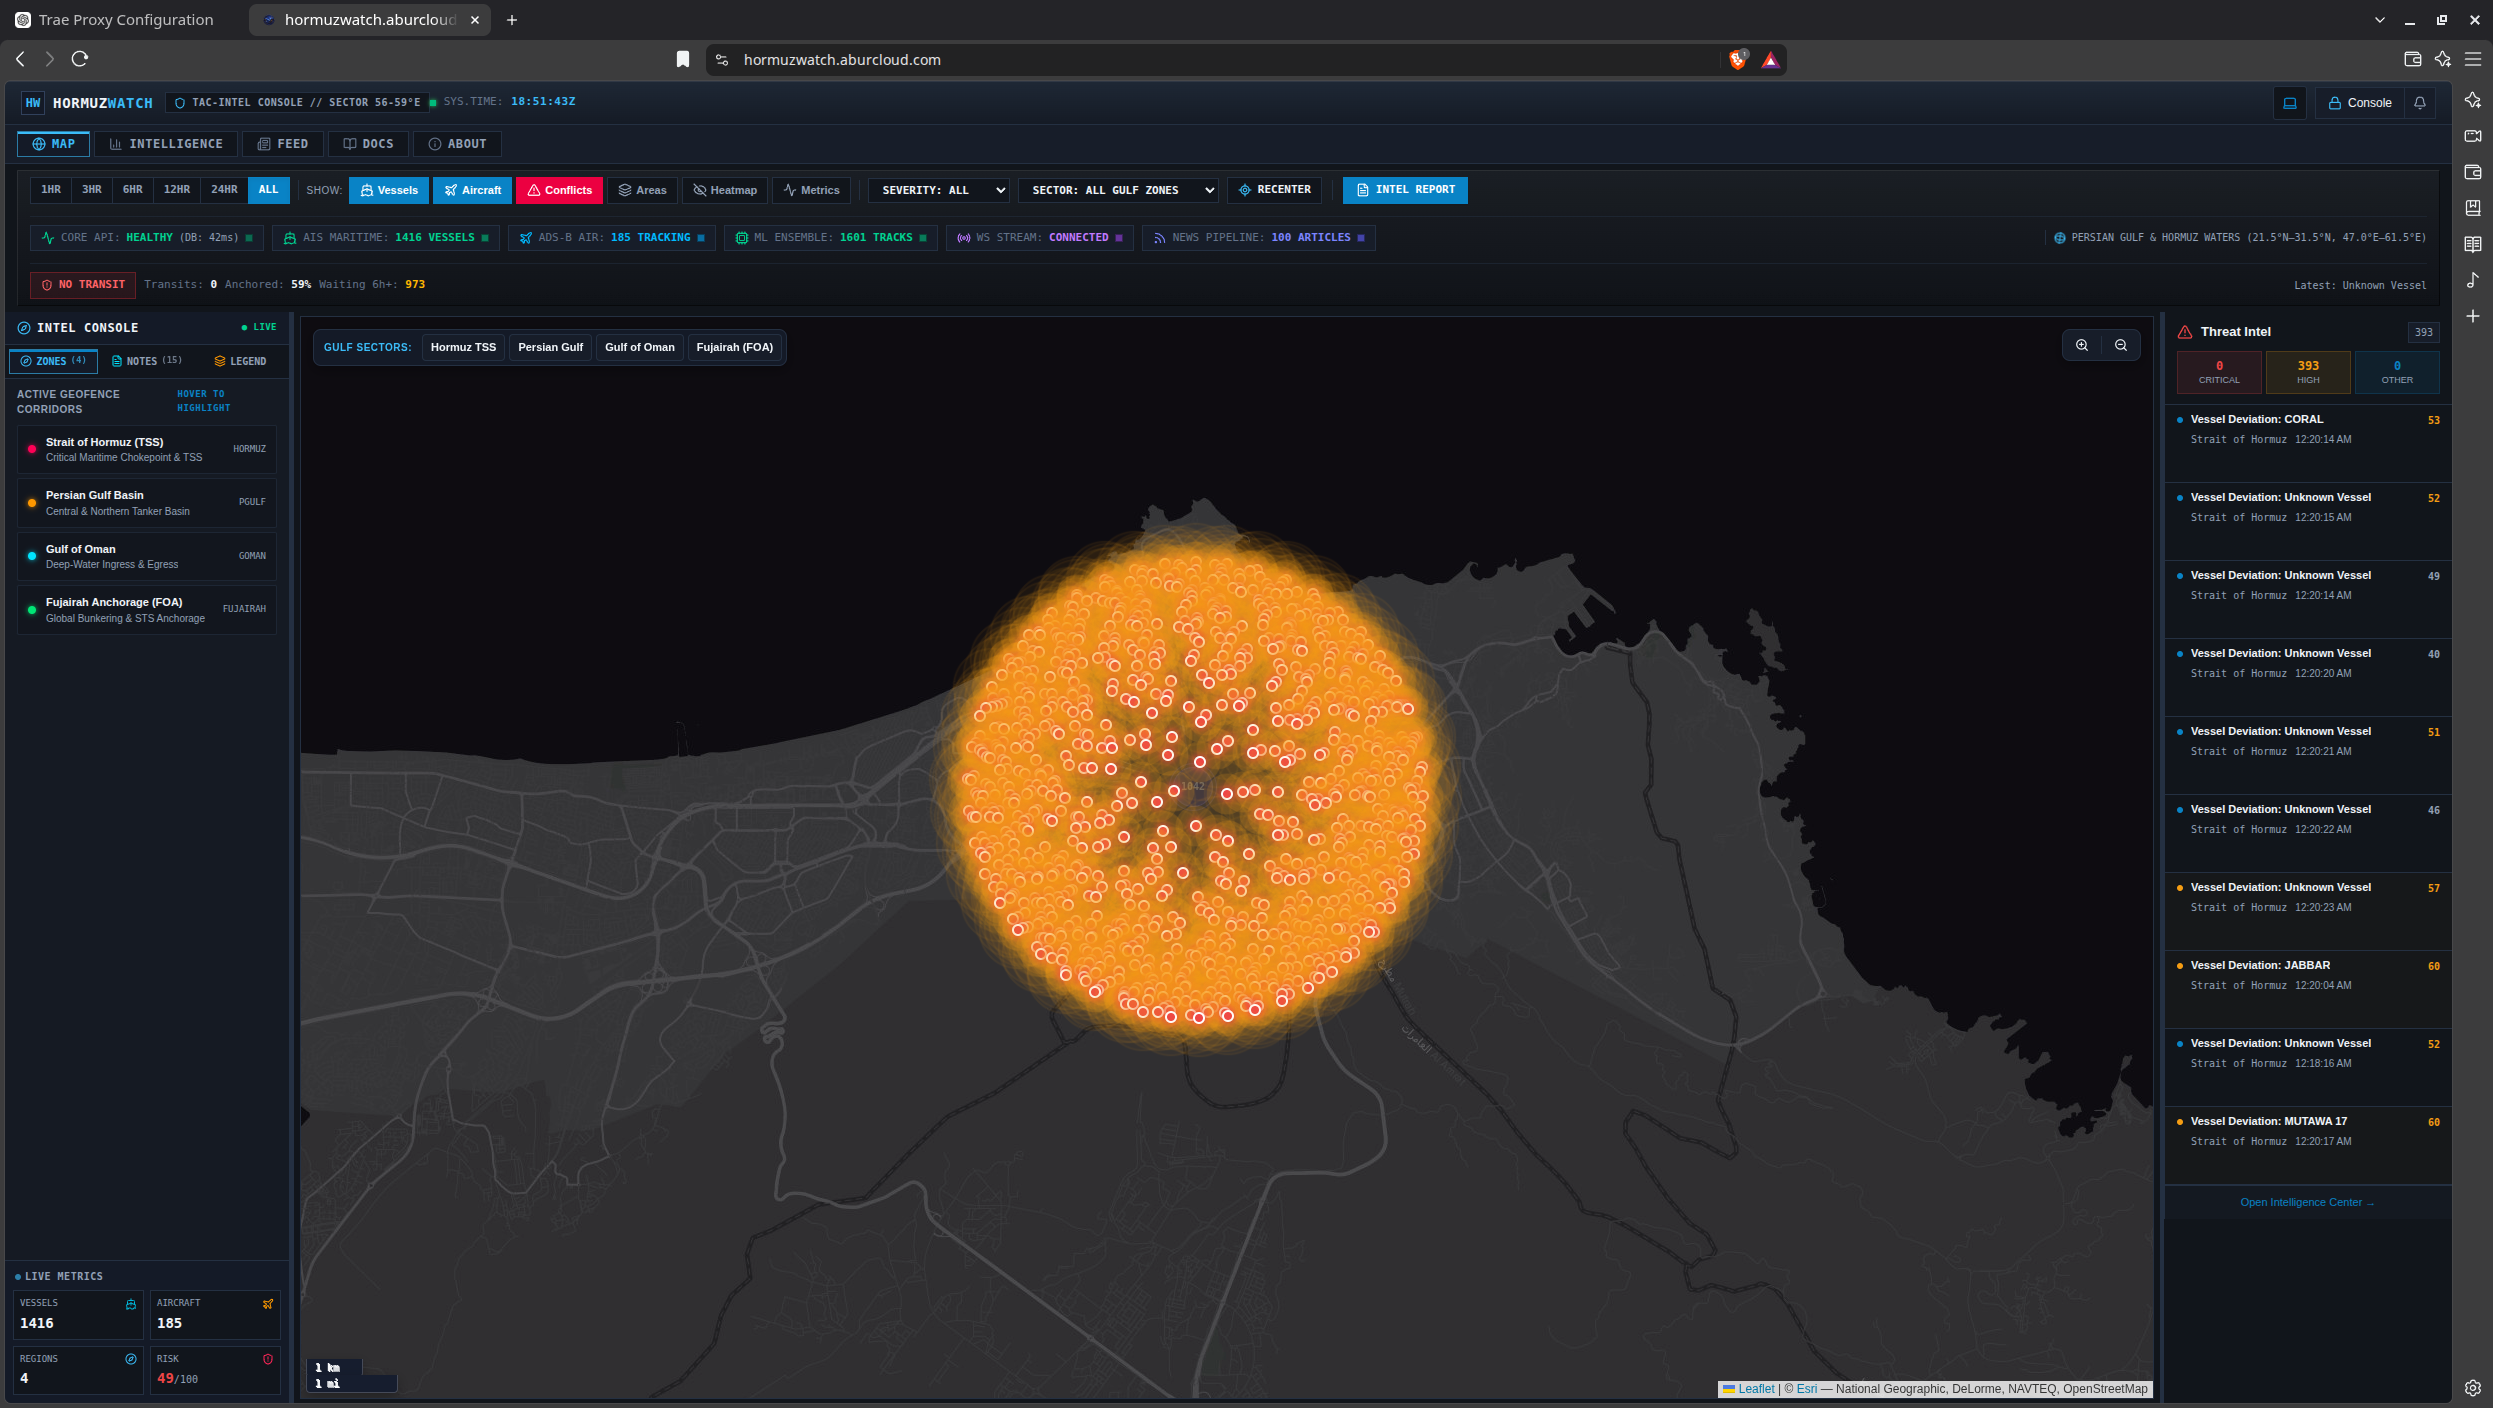
\includegraphics[width=0.92\textwidth]{figures/tactical_map_screenshot.png}
\caption{HormuzWatch Tactical Geospatial Interface displaying live maritime vessel tracking, Traffic Separation Schemes, and contact severity overlays.}
\label{fig:tactical_map}
\end{figure}

\subsubsection{Contact Dossier and Provenance Visualization}
When an operator selects an asset on the map, the custom Leaflet renderer dynamically constructs a tactical contact dossier popup (Figure~\ref{fig:app_window}):
\begin{figure}[htbp]
\centering

\includegraphics[width=0.88\textwidth]{figures/app_window_screenshot.png}
\caption{HormuzWatch Tactical Asset Dossier displaying real-time speed, heading, sector classification, AIS transponder health, and feed provenance metadata.}
\label{fig:app_window}
\end{figure}

\subsubsection{Multi-Domain Analytics and Telemetry Visualization}
Figure~\ref{fig:charts_viz} demonstrates the client-side telemetry analytics dashboard, projecting feature correlation distributions, speed variance trends, and temporal risk shifts across the maritime basin:
\begin{figure}[htbp]
\centering

\includegraphics[width=0.88\textwidth]{figures/charts_visualization.png}
\caption{HormuzWatch Telemetry Analytics Dashboard showing real-time speed variance, course deviation distributions, and multi-domain contact clusters.}
\label{fig:charts_viz}
\end{figure}
